\documentclass[hide notes,intlimits,usenames,dvipsnames]{beamer}

\mode<presentation>
{
  \usetheme{Singapore}
  \usefonttheme{professionalfonts}
  \setbeamertemplate{blocks}[rounded][shadow=true]
  \setbeamercovered{transparent}
  \setbeamertemplate{footline}[frame number]
}

% load packages
\usepackage[english]{babel}
\usepackage[latin1]{inputenc}
\usepackage[T1]{fontenc}
\usepackage{lmodern}
\usepackage[multidot]{grffile}
\usepackage{verbatim,empheq}

\usepackage{tikz}
\usetikzlibrary{shapes,arrows,shadows}
\usetikzlibrary{decorations.pathreplacing}

\usepackage{animate}
\usepackage{amsmath,verbatim}

% see http://tex.stackexchange.com/questions/86188/labelling-with-arrows-in-an-automated-way

\newif\ifclipme\clipmetrue
\tikzset{labelstyle/.style={LabelStyle/.append style={#1}},linestyle/.style={LineStyle/.append style={#1}}}
\tikzset{LabelStyle/.initial={},LineStyle/.initial={}}

\newcommand{\mathWithDescription}[4][]{{%
    \tikzset{#1}%
    \tikz[baseline]{
        \node[draw=red,rounded corners,anchor=base] (m#4) {$\displaystyle#2$};
        \ifclipme\begin{pgfinterruptboundingbox}\fi
            \node[above of=m#4,font=\strut, LabelStyle] (l#4) {#3};
            \draw[-,red, LineStyle] (l#4) to (m#4);
        \ifclipme\end{pgfinterruptboundingbox}\fi
    }%
}}

\newcommand{\mathWithDescriptionStarred}[3][]{{%
    \clipmefalse%
    \mathWithDescription[#1]{#2}{#3}{\themathLabelNode}%
}}

\newcounter{mathLabelNode}

\newcommand{\mathLabelBox}[3][]{%
   \stepcounter{mathLabelNode}%
   \mathWithDescription[#1]{#2}{#3}{\themathLabelNode}%
   \vphantom{\mathWithDescriptionStarred[#1]{#2}{#3}{\themathLabelNode}}%
}

\definecolor{dark red}{HTML}{E41A1C}
\definecolor{dark green}{HTML}{4DAF4A}
\definecolor{dark violet}{HTML}{984EA3}
\definecolor{dark blue}{HTML}{084594}
\definecolor{dark orange}{HTML}{FF7F00}
\definecolor{light blue}{HTML}{377EB8}
\definecolor{light red}{HTML}{FB9A99}
\definecolor{light violet}{HTML}{CAB2D6}

\newcommand{\CC}{\mathbb{C}}
\newcommand{\NN}{\mathbb{N}}
\newcommand{\RR}{\mathbb{R}}
\newcommand{\ZZ}{\mathbb{Z}}

\newcommand{\Kcal}{\mathcal{K}}
\newcommand{\Xcal}{\mathcal{X}}

\newcommand{\bF}{\mathbf{F}}
\newcommand{\bQ}{\mathbf{Q}}
\newcommand{\bU}{\mathbf{U}}
\newcommand{\bX}{\mathbf{X}}

\newcommand{\bn}{\mathbf{n}}
\newcommand{\bq}{\mathbf{q}}
\newcommand{\bu}{\mathbf{u}}
\newcommand{\bv}{\mathbf{v}}
\newcommand{\bx}{\mathbf{x}}

\newcommand{\Div}{\nabla\cdot}
\newcommand{\eps}{\epsilon}
\newcommand{\grad}{\nabla}
\newcommand{\lap}{\triangle}
\renewcommand{\bar}{\overline}

\newcommand{\ip}[2]{\ensuremath{\left<#1,#2\right>}}


\newenvironment{transbox}[1][]{%
\begin{tikzpicture}
\node[drop shadow,rounded corners,text width=\textwidth,fill=white, fill opacity=#1,text opacity=1] \bgroup
}{
\egroup;\end{tikzpicture}}


\title{A practical view of the FEM}

\subtitle{with some software}

\author[Bueler]{Ed Bueler}

\institute[UAF]{
  \scriptsize Dept of Mathematics and Statistics \\

  University of Alaska Fairbanks
}

%\titlegraphic{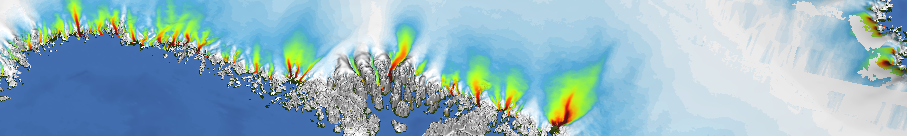
\includegraphics[width=\textwidth]{andycoast.png}}

\beamertemplatenavigationsymbolsempty   % remove faint and silly navigation symbols at bottom
\renewcommand{\insertnavigation}[1]{}   % remove section headings from top of each slide

\setbeamerfont{date}{size=\scriptsize}
\date{}

%\AtBeginSection[]
%{
%  \begin{frame}<beamer>
%    \frametitle{Outline}
%    %\tableofcontents[currentsection,hideallsubsections]
%    \tableofcontents[currentsection]
%  \end{frame}
%}


\begin{document}

\begin{frame}
\vspace{10mm}
  \titlepage
  \begin{center}
  \tiny DMS \hfill 27 November 2018
  \end{center}
\end{frame}


\begin{frame}
    \frametitle{Outline}
    \tableofcontents
\end{frame}

\section{assembly}

\begin{frame}{general Poisson problem}
\begin{itemize}
\item everything today is in 2D
\item consider a generalization of our usual ``$\triangle u = f$, $u=0$ on $\partial\Omega$'' problem:
\begin{align}
- \Div \left(a(u) \grad u\right) &= f(u)  &&\text{ on } \Omega, \label{eq:un:poissonstrong} \\
u &= g_D &&\text{ on } \partial_D \Omega, \notag \\
\frac{\partial u}{\partial n} &= g_N &&\text{ on } \partial_N \Omega. \notag
\end{align}
\item we assume \emph{uniform ellipticity}
\begin{equation}
a(u,x,y) \ge \eps > 0, \label{eq:un:uniformelliptic}
\end{equation}
\item and that $f(u,x,y)$ and $g_N(x,y)$ and $g_D(x,y)$ are given continuous (or at least $L^2$) functions
\end{itemize}
\end{frame}

\begin{frame}{general Poisson problem}
\begin{center}
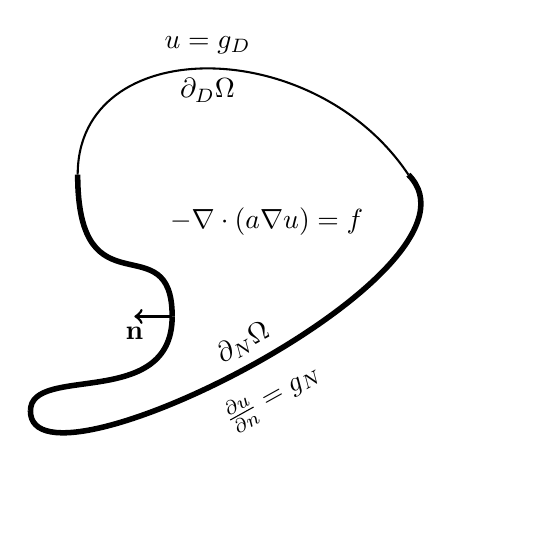
\begin{tikzpicture}[scale=0.6]
\draw[line width=0.75pt] (0,0) .. controls (0,3) and (5,3) .. node[sloped,above,yshift=0.5mm] {$u=g_D$} node[sloped,below] {$\partial_D\Omega$} (7,0);
\draw[line width=2pt] (7,0) .. controls (9,-2) and (-1,-7) .. node[sloped,above] {$\partial_N\Omega$} node[sloped,below,yshift=-1mm] {$\frac{\partial u}{\partial n} = g_N$} (-1,-5);
\draw[line width=2pt] (-1,-5) .. controls (-1,-4) and (2,-5) .. (2,-3);
\draw[line width=2pt] (2,-3) .. controls (2,-1) and (0,-3) .. (0,0);
\draw[->,line width=1.0pt] (2,-3) -- (1.2,-3) node[below] {$\bn$}; % normal vector
\draw (4,-1) node {$- \Div (a \grad u) = f$};
\end{tikzpicture}


\end{center}
\end{frame}

\begin{frame}{X}
X
\end{frame}

\begin{frame}{X}
X
\end{frame}

\begin{frame}{X}
X
\end{frame}

\section{solving the equations}

\begin{frame}{X}
X
\end{frame}

\begin{frame}{X}
X
\end{frame}

\section{runtime choices}

\begin{frame}{X}
X
\end{frame}

\begin{frame}{X}
X
\end{frame}

\begin{frame}{X}
X
\end{frame}

\begin{frame}{X}
X
\end{frame}

\begin{frame}{X}
X
\end{frame}

\begin{frame}{X}
X
\end{frame}


\end{document}
